% $Id: INF_Poster.tex 7714 2011-08-31 17:34:46Z tkren $
%
% TU Wien - Faculty of Informatics
% poster template
%
% This template is using the beamer document class and beamerposter package, see
% <http://www.ctan.org/tex-archive/macros/latex/contrib/beamer/>
% <http://www.ctan.org/tex-archive/macros/latex/contrib/beamerposter/>
% <http://www-i6.informatik.rwth-aachen.de/~dreuw/latexbeamerposter.php>
%
% For questions and comments send an email to
% Thomas Krennwallner <tkren@kr.tuwien.ac.at>
%

\documentclass[final,hyperref={pdfpagelabels=false}]{beamer}

\usepackage{TUINFPST}

\title[Computational Intelligence]{Design and Implementation of an Agent Architecture combining Emotions and Reasoning}
\author[janos.tapolczai@alumni.tuwien.ac.at]{Janos Tapolczai}
\institute[]{%
    Technische Universit{\"a}t Wien\\[0.25\baselineskip]
    Institut f{\"u}r Informationssysteme 184/3\\[0.25\baselineskip]
    Arbeitsbereich: Knowledge Based Systems\\[0.25\baselineskip]
    BetreuerIn: a.o. Univ.-Prof. Dr. Hans Tompits\\[0.25\baselineskip]
}
\titlegraphic{
\includegraphics[height=52mm]{kbs-logo}}
\date[\today]{\today}
\subject{epilog}
\keywords{artificial intelligence, reasoning, affective}

%%%%%%%%%%%%%%%%%%%%%%%%%%%%%%%%%%%%%%%%%%%%%%%%%%%%%%%%%%%%%%%%%%%%%%%%%%%%%%%%%%%%%%
% Display a grid to help align images 
%\beamertemplategridbackground[1cm]

% play around with the background colors
% \setbeamercolor{background canvas}{bg=yellow}

% use a background picture
% \usebackgroundtemplate{%
%   
\includegraphics[width=\paperwidth]{logo_KBS_2_CMYK}
% }

% play around with block colors
\setbeamercolor{block body}{fg=black,bg=white}
\setbeamercolor{block title}{fg=TuWienBlue,bg=white}

\setbeamertemplate{block begin}{
    \begin{beamercolorbox}{block title}%
        
\begin{tikzpicture}%
        \node[draw,rectangle,line width=3pt,rounded corners=0pt,inner sep=0pt]{%
            \begin{minipage}[c][2cm]{\linewidth}
            \centering\textbf{\insertblocktitle}
            \end{minipage}
        };
        \end{tikzpicture}%
    \end{beamercolorbox}
    \vspace*{1cm}
    \begin{beamercolorbox}{block body}%
}
    
\setbeamertemplate{block end}{
    \end{beamercolorbox}
    \vspace{2cm}
}

% setup postit
\setbeamercolor{postit}{fg=black,bg=yellow} 
\newenvironment{postit}
{\begin{beamercolorbox}[sep=1em,wd=7cm]{postit}}
{\end{beamercolorbox}}

% for crop marks, uncomment the following line
%\usepackage[cross,width=88truecm,height=123truecm,center]{crop}

% setup url size
\usepackage{url}
\urlstyle{same}

% setup download links
\usepackage{wrapfig}
\usepackage{qrcode}

% setup bibliography
\bibliographystyle{plain}

%%%%%%%%%%%%%%%%%%%%%%%%%%%%%%%%%%%%%%%%%%%%%%%%%%%%%%%%%%%%%%%%%%%%%%%%%%%%%%%%%%%%%%

\begin{document}

% We have a single poster frame.
\begin{frame}
    \begin{columns}[t]
        % ---------------------------------------------------------%
        % Set up a column
        \begin{column}{.45\textwidth}
            \begin{block}{Introduction \& Problem Statement}                
                \begin{itemize}
                    \item Reasoning and search can explore solution spaces, but they can't tell an agent which goals it should value.
                    \item Often, outcomes are valued via goal functions and are categorized into ``good'' and ``bad'' ones, depending on the value of the function.
                    \item Can one combine simple emotional reactions to situations with reasoning techniques to obtain intelligent behaviour?
                \end{itemize}
                
                $~$
                
                \textbf{Wumpus World}\\
                As our setting, we chose and elaborate version of the well-known Wumpus world: a 2D-grid world with Wumpuses that try to kill agents, plants that can be harvested, and items that can be picked up. Agents have to avoid being killed and have to periodically eat either the fruit from plants or the meat from Wumpuses whom they can fight.
            \end{block}
            
            \begin{block}{Combining Affect and Reasoning}                
                We have created an AI consisting of loosely coupled components that communicate via a central message space.
                
                $~$
                
                \textbf{Structure}
                \begin{itemize}
                	\item Agents emotionally evaluate their current situation and take a hypothetical action based on the strongest emotion.
                	\item The world is simulated one step ahead.
                	\item If the outcome satisfies the strongest emotion, the action is actually taken.
                	\item If not, the planning continues or a different action is tried.
                \end{itemize}
                
                $~$
                
                \textbf{Emotions}
                \begin{itemize}
                	\item Evolutionarily speaking, organisms felt fear and anger long before they felt social emotions.
                	\item We thus divided the emotions into pre-social and social ones.
                	\item The pre-social emotions are put into four categories based on neurological research: anger, fear, enthusiasm, contentment.
                	\item Anger is negative and approach-related,
                	\item Fear is negative and avoidance-related.
                	\item Enthusiasm is positive and approach-related,
                	\item Contentment is negative and avoidance-related, inasmuch as it leads the organism to avoid action because its needs are met.
                \end{itemize}
                
                $~$
                
                \begin{figure}
                	\centering
                	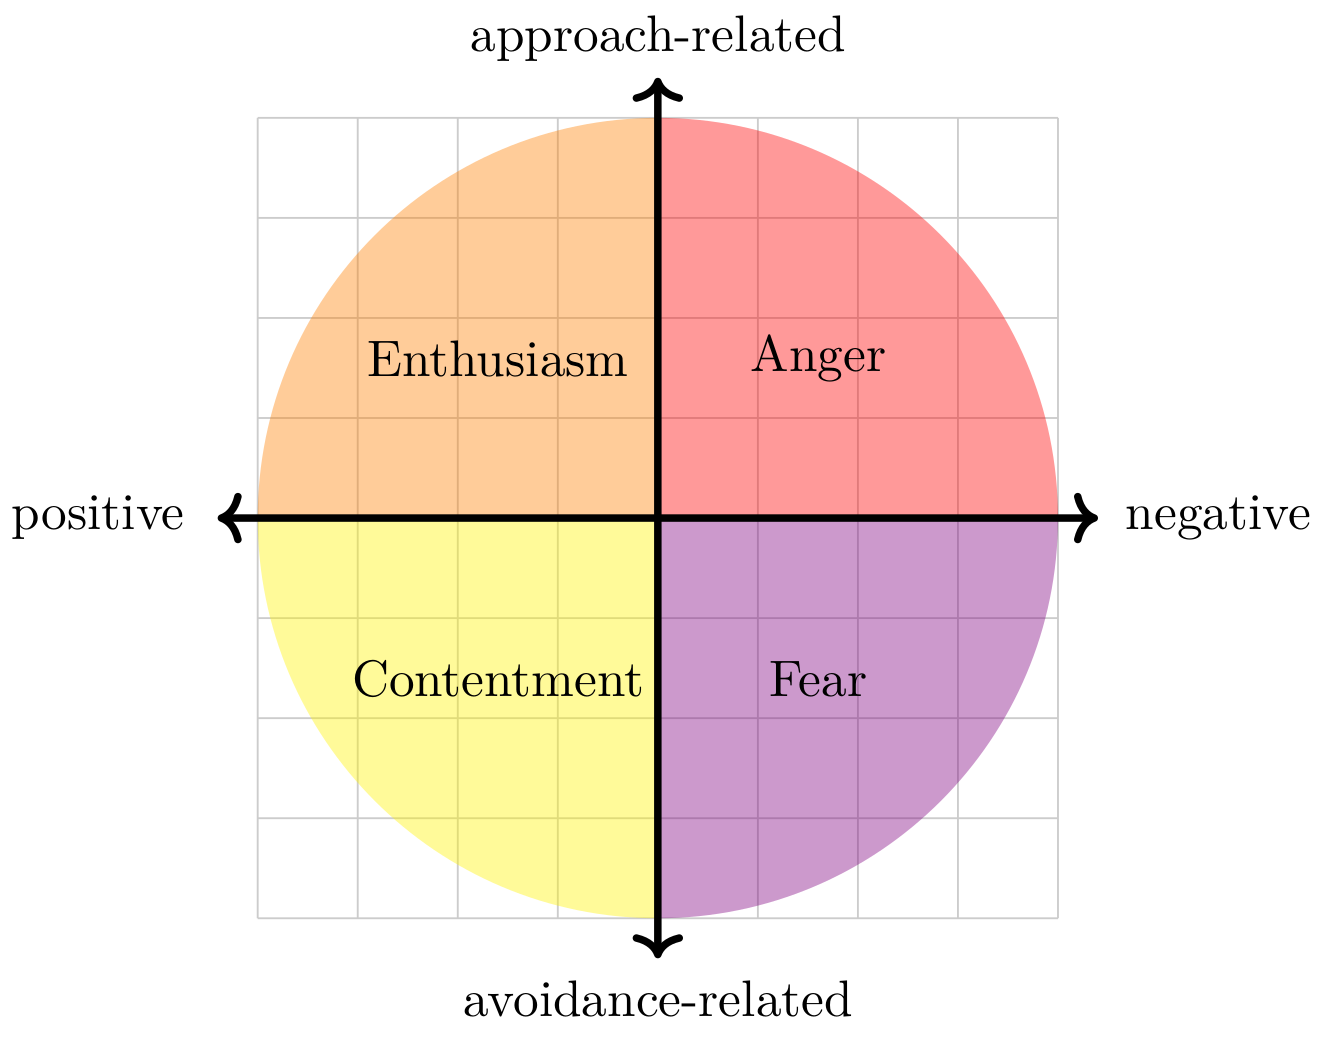
\includegraphics[width=0.75\textwidth]{figures/psbc.png}
                \end{figure}
            \end{block}
        \end{column}
        % ---------------------------------------------------------%
        % end the column
        
        % ---------------------------------------------------------%
        % Set up a column 
        \begin{column}{.45\textwidth}            
            \begin{block}{Proof of Concept}
            	We wrote a proof of the concept Haskell. The two major components are the world simulation and the AI.
                
                $~$
                
                \textbf{World simulation}
                \begin{itemize}
                    \item Implements the semantics of the Wumpus world.
                    \item Offers a number of actions: rotate, move, pick up item, give item, attack etc.
                    \item Provides agents with perceptions: visual data, breeze from pits, stench from Wumpuses, location, direction.
                    \item Treats AIs as black boxes that need only implement a \texttt{getAction}-function.
                \end{itemize}
                
                $~$
                
                \textbf{AI}
                \begin{itemize}
                    \item Consists of loosely coupled components that communicate via a shared message space.
                    \item Components are called sequentially in each round.
                    \item Each component can read the previous messages and insert its own.
                    \item The pre-social behaviour control (PSBC) and social judgment system (SJS) provide emotional reactions.
                    \item The decision makes takes hypothetical or real actions.
                    \item The belief generator simulates the consequences of actions.
                    \item The attention module selects important targets like fruit or nearby hostile agents.
                \end{itemize}
                
                $~$
                
                \begin{figure}
                	\centering
                	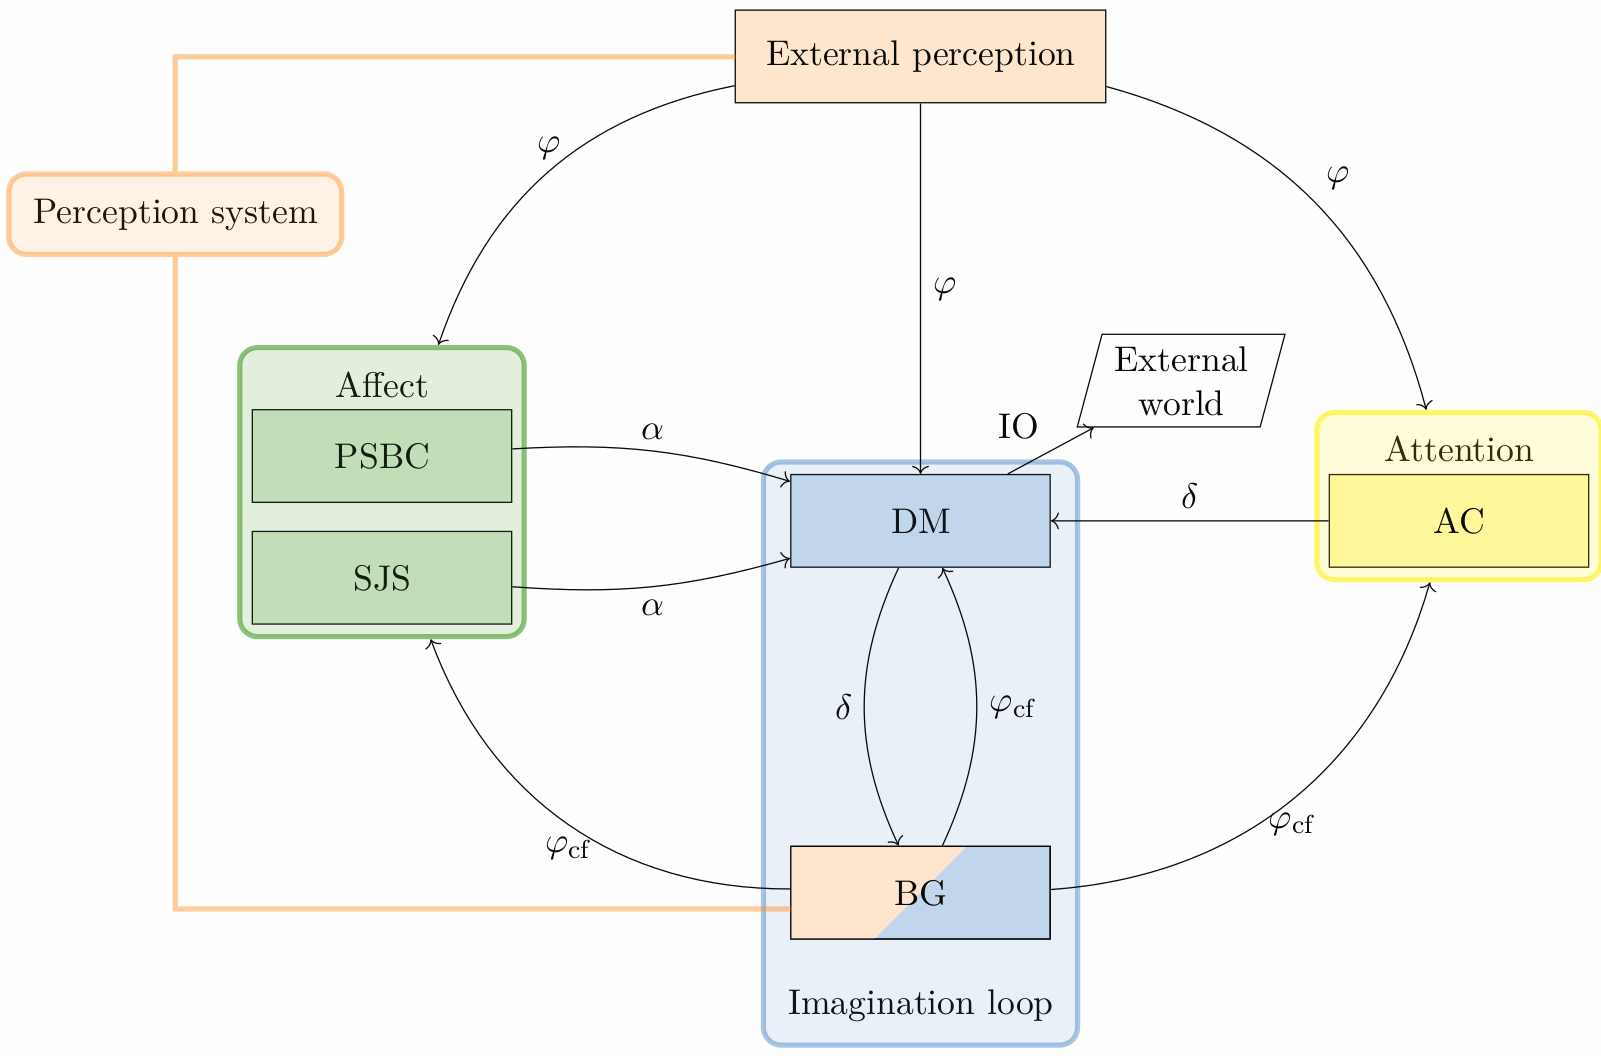
\includegraphics[width=0.75\textwidth]{figures/architecture.png}
                \end{figure}
            \end{block}
            
            \begin{block}{Evaluation}
                We put the AIs in a number of test worlds to see whether they would perform reasonable actions:
                \begin{itemize}
                    \item Harvesting a plant and eating its fruit when hungry,
                    \item Fleeing from a Wumpus when low on health.
                    \item Attacking a Wumpus when in good health.
                \end{itemize}
            \end{block}
            
            \begin{block}{Conclusion}
                % use columns so we can print the download link to the right
                \begin{columns}[t]
                    \begin{column}{0.77\textwidth}
                        \begin{itemize}
                            \item We created a hybrid AI that combines emotions and reasoning.
                            \item There are no explicit goal functions, only conflicting emotions.
                            \item The AI performs well on rudimentary tasks.
                        \end{itemize}
                    \end{column}
                    % print the download link
                    \begin{column}{0.23\textwidth}
                        \begin{block}{DOWNLOAD}
                            \begin{center}
                                \qrcode[hyperlink,height=2.5in]{https://github.com/jtapolczai/wumpus}
                        \end{center}
                        \end{block}
                    \end{column}
                \end{columns}
            \end{block}
        \end{column}
        % ---------------------------------------------------------%
        % end the column
    \end{columns}
\end{frame}

\end{document}

%%% Local Variables:
%%% TeX-PDF-mode: t
%%% TeX-debug-bad-boxes: t
%%% TeX-master: t
%%% TeX-parse-self: t
%%% TeX-auto-save: t
%%% reftex-plug-into-AUCTeX: t
%%% End:
